%
% $RCSfile: virtual_and_real_world.tex,v $
%
% Copyright (C) 2002-2008. Christian Heller.
%
% Permission is granted to copy, distribute and/or modify this document
% under the terms of the GNU Free Documentation License, Version 1.1 or
% any later version published by the Free Software Foundation; with no
% Invariant Sections, with no Front-Cover Texts and with no Back-Cover
% Texts. A copy of the license is included in the section entitled
% "GNU Free Documentation License".
%
% http://www.cybop.net
% - Cybernetics Oriented Programming -
%
% http://www.resmedicinae.org
% - Information in Medicine -
%
% Version: $Revision: 1.1 $ $Date: 2008-08-19 20:41:09 $ $Author: christian $
% Authors: Christian Heller <christian.heller@tuxtax.de>
%

\section{Virtual- and Real World}
\label{virtual_and_real_world_heading}
\index{Virtual- and Real World}

A separate treatment of knowledge and system functionality can be observed in
many fields of science. Some examples are given following.

%
% $RCSfile: mind_and_body.tex,v $
%
% Copyright (C) 2002-2008. Christian Heller.
%
% Permission is granted to copy, distribute and/or modify this document
% under the terms of the GNU Free Documentation License, Version 1.1 or
% any later version published by the Free Software Foundation; with no
% Invariant Sections, with no Front-Cover Texts and with no Back-Cover
% Texts. A copy of the license is included in the section entitled
% "GNU Free Documentation License".
%
% http://www.cybop.net
% - Cybernetics Oriented Programming -
%
% http://www.resmedicinae.org
% - Information in Medicine -
%
% Version: $Revision: 1.1 $ $Date: 2008-08-19 20:41:07 $ $Author: christian $
% Authors: Christian Heller <christian.heller@tuxtax.de>
%

\subsection{Mind and Body}
\label{mind_and_body_heading}
\index{Mind and Body}
\index{Philosophy}
\index{Metaphysics}
\index{Ontology}
\index{Knowledge}
\index{Dualism}
\index{Being}
\index{Hardware}
\index{Software}
\index{Operating System}
\index{OS}

In \emph{Philosophy}, it is common to distinguish between two traditions:
Euro-American \emph{Western Philosophy} and Asian \emph{Eastern Philosophy}
\cite{wikipedia}. The former, also called \emph{Western Academic Philosophy},
is often divided into: \emph{Analytic-} and \emph{Continental Philosophy}.
While continental philosophy is predominant in continental Europe, analytic
philosophy dominates Anglo-American philosophy. Western philosophy has its
roots in ancient \emph{Greek Philosophy}, which, among others, dealt with five
broad types of analytical questions \cite{wikipedia}:

\begin{itemize}
    \item[-] \emph{metaphysical:} study of any of the most fundamental concepts
        and beliefs about the basic nature of \emph{Reality}, such as
        \emph{Ontology} as the science of \emph{Being}
    \item[-] \emph{epistemological:} study of the nature, origin and scope of
        \emph{Knowledge}
    \item[-] \emph{logical:} study of \emph{Inference}, that is \emph{Reasoning}
        used to reach a conclusion from a set of assumptions
    \item[-] \emph{ethical:} study of \emph{Morality}, that is behaviour which
        is \emph{good}
    \item[-] \emph{aesthetic:} study of the nature of \emph{Beauty}
\end{itemize}

To the metaphysical questions belong:

\begin{itemize}
    \item[-] What is reality, and what things can be described as real?
    \item[-] What is the nature of those things?
    \item[-] Do some things exist independently of our perception?
    \item[-] What is the nature of space and time?
    \item[-] What is the nature of thought and thinking?
    \item[-] What is it to be a person?
\end{itemize}

As already mentioned in section \ref{ontos_and_logos_heading}, ontology and
metaphysics are closely related. The Skeptic's Dictionary
\cite{skepticsdictionary} writes:

\begin{quote}
    \emph{Ontology} is a branch of \emph{Metaphysics} which is concerned with
    being, including theories of the nature and kinds of being. \emph{Monistic}
    ontologies hold that there is only one being, such as Spinoza's theory that
    God or Nature is the only substance. \emph{Pluralistic} ontologies hold that
    there is no unity to being and that there are numerous kinds of being.
    \emph{Dualism} is a kind of pluralistic ontology, maintaining that there
    are two fundamental kinds of being: \emph{Mind} and \emph{Body}.
\end{quote}

The question how both are related is known as \emph{Mind-Body-Problem}, and
besides the above-mentioned pluralistic \emph{Dualism}, there are two monistic
views to it \cite{wikipedia}:

\begin{itemize}
    \item[-] \emph{Materialism} (\emph{Physicalism}) is the view that mental
        events are nothing more than a special kind of physical event
    \item[-] \emph{Phenomenalism} (\emph{Subjective Idealism}) is the view that
        physical events are nothing more than a special kind of mental event
\end{itemize}

\newpage

The Wikipedia encyclopedia \cite{wikipedia} writes:

\begin{quote}
    Most neuroscientists believe in the identity of mind and brain, a position
    that may be considered related to materialism and physicalism, though there
    is a subtle difference; namely, that postulating an identity between mind
    and brain (or more specifically, particular types of neuronal interactions)
    does not necessarily imply that mental events are \emph{nothing more} than
    physical events, but rather is more akin to saying that physical events and
    mental events are different aspects of a more fundamental mental-physical
    substratum which can be perceived as both mental and physical, depending on
    perspective.
\end{quote}

The idea described hereafter follows this interpretation of materialism.
Applied to human existence, this philosophical perspective means that the mind
of human systems carries a \emph{Virtual World} that is supposed to be formed
by the activity of an underlying physical brain, which serves as representation
within the \emph{Real World}. Other questions like whether human systems also
host something like a \emph{Soul}, or if the mind actually is what makes up the
soul are a topic of \emph{Religion} and not further discussed here.

Transferring this philosophical view to information engineering, one might at
first think that \emph{Hardware} is what represents the body- and
\emph{Software} what represents the mind of a computer system. This is true in
the first instance, but not thought through to the end. There are many kinds of
software. \emph{Operating Systems} (OS) with their \emph{Device Drivers},
\emph{Embedded Systems}, \emph{Real Time Systems} or \emph{Firmware} operate
close to hardware. \emph{Standard-} and \emph{Business Applications}, on the
other hand, contain a lot of logic and domain knowledge which is independent
from the underlying hardware.

As result, one might as well treat hardware \emph{together} with
hardware-dependent system control software as the body-, and pure application
knowledge as mind of a computer system. While system control requires some
\emph{active} software running a process (section \ref{process_heading}) or
threads and controlling devices, application knowledge may absolutely be
\emph{passive}.

One argument in favour of summarising hardware and system control software was
mentioned in section \ref{paradigm_and_language_heading} which cited Tanenbaum
\cite{tanenbaum1999} who considers hardware and software to be
\textit{logically equivalent} because one could replace the other.

%
% $RCSfile: brain_regions.tex,v $
%
% Copyright (C) 2002-2008. Christian Heller.
%
% Permission is granted to copy, distribute and/or modify this document
% under the terms of the GNU Free Documentation License, Version 1.1 or
% any later version published by the Free Software Foundation; with no
% Invariant Sections, with no Front-Cover Texts and with no Back-Cover
% Texts. A copy of the license is included in the section entitled
% "GNU Free Documentation License".
%
% http://www.cybop.net
% - Cybernetics Oriented Programming -
%
% http://www.resmedicinae.org
% - Information in Medicine -
%
% Version: $Revision: 1.1 $ $Date: 2008-08-19 20:41:05 $ $Author: christian $
% Authors: Christian Heller <christian.heller@tuxtax.de>
%

\subsection{Brain Regions}
\label{brain_regions_heading}
\index{Brain Regions}
\index{Central Nervous System}
\index{CNS}
\index{Peripheral Nervous System}
\index{PNS}

\emph{Neurology} as branch of \emph{Medicine} deals with the
\emph{Central Nervous System} (CNS) and \emph{Peripheral Nervous System} (PNS)
of human beings. These can be further divided as shown in figure
\ref{nervoussystem_figure}.

\begin{figure}[ht]
    \begin{center}
        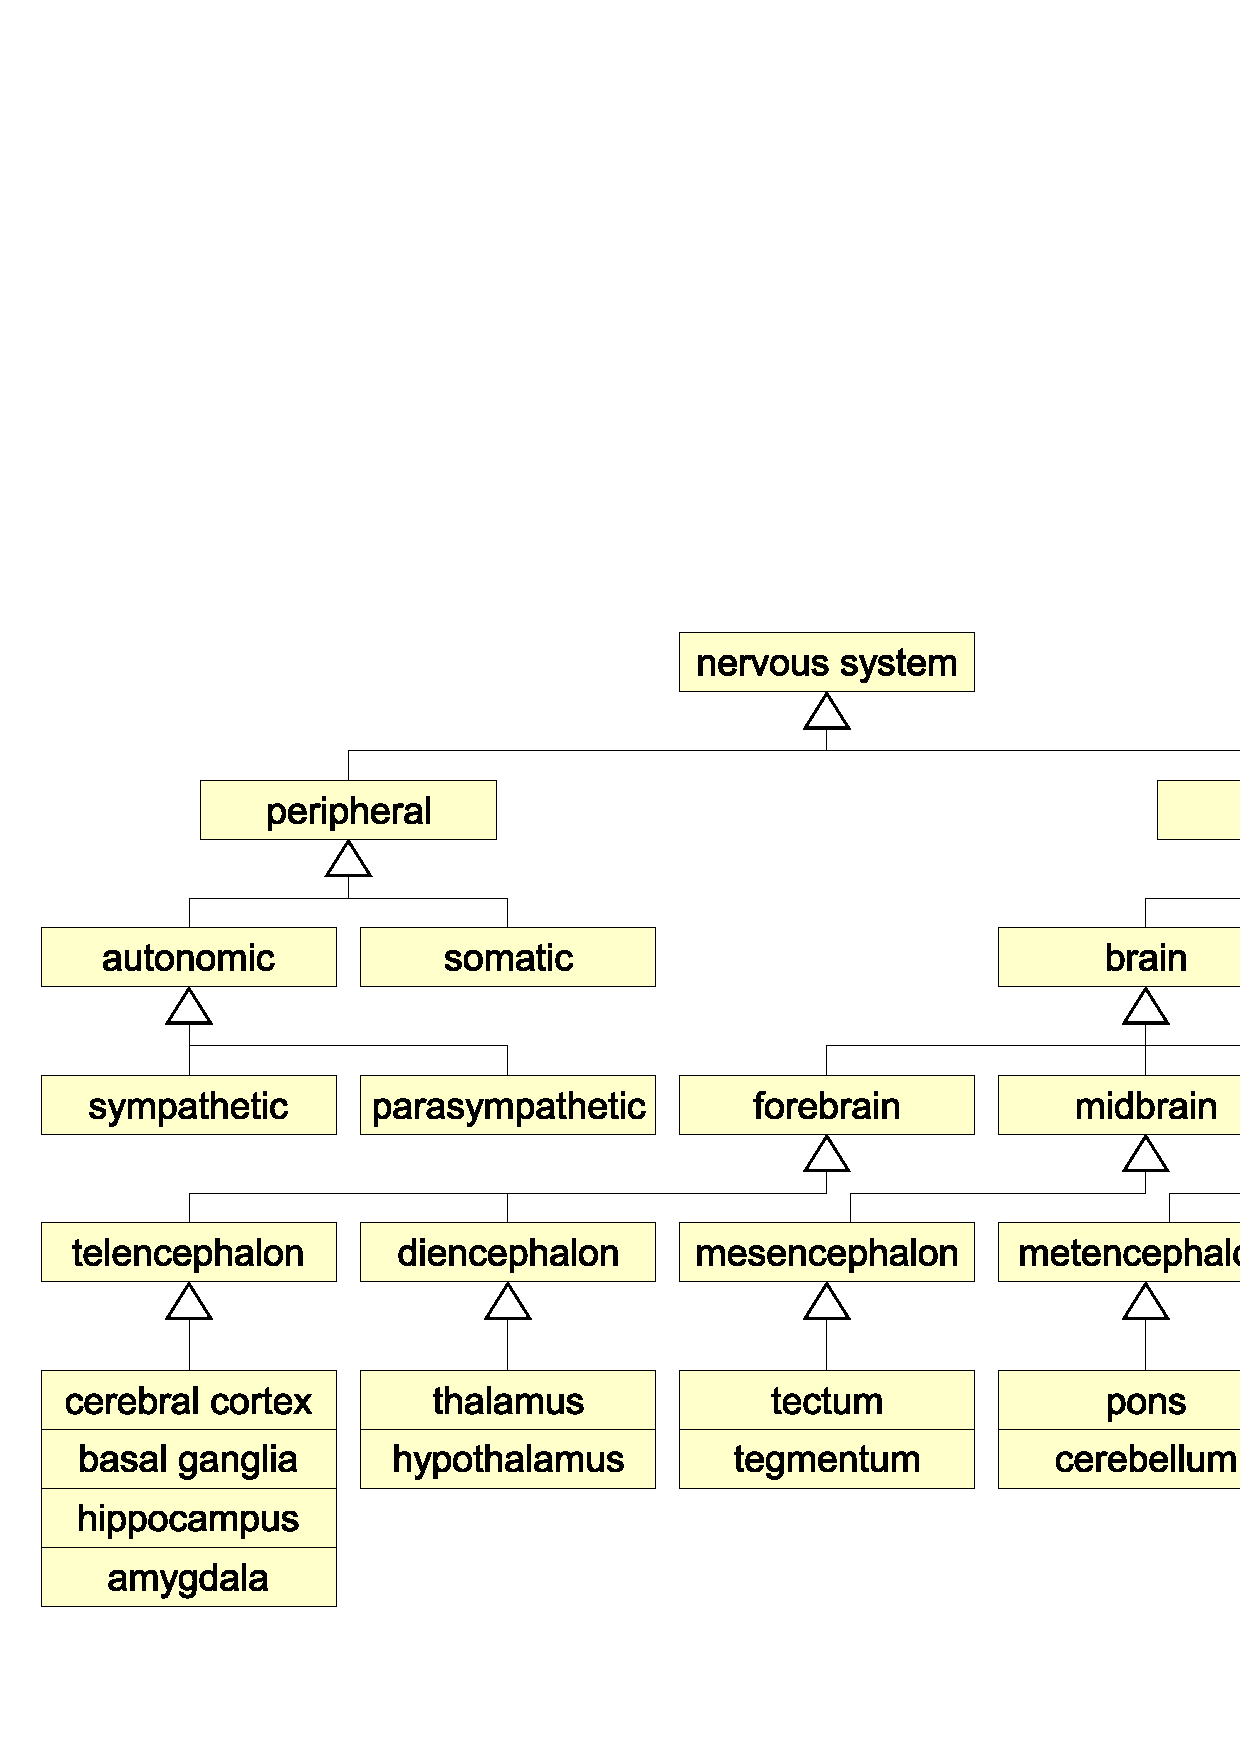
\includegraphics[scale=0.3,angle=-90]{graphic/nervoussystem.pdf}
        \caption{Divisions of the Nervous System \cite{adventuresinneuroanatomy}}
        \label{nervoussystem_figure}
    \end{center}
\end{figure}

Not all parts of this systematics shall be explained here; more details can be
found at \cite{pschyrembel}. Chapter \ref{state_and_logic_heading} will make
some remarks on the PNS, whose \emph{Neurons} (nerve cells) can be functionally
divided into \emph{sensory} (\emph{afferent}) and \emph{motor}
(\emph{efferent}) ones. The functions of some brain structures, as part of the
CNS, are described in table \ref{brainstructures_table}. At the same time, this
table (where \emph{n/a} means \emph{not applicable}) tries to give possible
analogies to a standard computer system, whereby hardware as well as software
are considered.

\begin{table}[ht]
    \begin{center}
        \begin{footnotesize}
        \begin{tabular}{| p{25mm} | p{50mm} | p{30mm} |}
            \hline
            \textbf{Brain Structure} & \textbf{Function} & \textbf{Computer Analogon}\\
            \hline
            Cerebral Cortex
            & Thought, Voluntary Movement, Language, Reasoning, Perception
            & Application/ Domain Knowledge\\
            \hline
            Cerebellum
            & Movement, Balance, Posture
            & n/a (only in Robots)\\
            \hline
            Brain Stem %(medulla, pons, tectum, tegmentum)
            & Breathing, Heart Rate, Blood Pressure
            & Timer, Power Supply\\
            \hline
            Hypothalamus
            & Body Temperature, Hunger, Thirst, Emotions, Circadian Rhythms
            & Self-observing Sensors (Battery-/ CPU Status)\\
            \hline
            Thalamus
            & Sensory Processing, Information Forwarding, Movement
            %(cerebral cortex [forwards information] to other brain areas and spinal cord)
            & Event Mechanism, Signal Loop, IRQ Handler\\
            \hline
            Limbic System %(amygdala, hippocampus)
            & Emotions
            & Signal Priorities\\
            \hline
            Hippocampus
            & Learning, Memory
            & Knowledge Storage, RAM\\
            \hline
            Basal Ganglia %(globus pallidus, caudate nucleus,
            %subthalamic nucleus, putamen, substantia nigra)
            & Movement
            & n/a (only in Robots)\\
            \hline
            Midbrain %(superior/ inferior colliculi, red nucleus)
            & Vision, Audition, Eye- and Body Movement
            & I/O Device Drivers, Translation\\
            \hline
        \end{tabular}
        \end{footnotesize}
        \caption{Brain Structures in Analogy to a Computer \cite{adventuresinneuroanatomy}}
        \label{brainstructures_table}
    \end{center}
\end{table}

Of course, the analogies do not match exactly. Also, there are many functions
-- like \emph{Thought} or \emph{Emotions} -- that a computer cannot perform.
The important thing to notice, however, is that there are brain regions mainly
\emph{storing} (Hippocampus) and \emph{applying} knowledge (Cerebral Cortex) and
others \emph{coordinating} the input/ output (i/o) of that knowledge (Midbrain,
Basal Ganglia) in form of simplified information, through sensoric/ motoric
organs of the human body.

That is, what philosophy calls \emph{Mind} (section \ref{mind_and_body_heading})
is the \emph{Knowledge} that is anatomically-physically mainly situated in the
\emph{Hippocampus} and \emph{Cerebral Cortex}. And again, i/o control does not
only rely on hardware devices but also on the corresponding driver software and
signalling mechanism. To say it differently: The software that contains
application/ domain knowledge is to be treated \emph{separately} from system
control software.

%
% $RCSfile: cell_division.tex,v $
%
% Copyright (C) 2002-2008. Christian Heller.
%
% Permission is granted to copy, distribute and/or modify this document
% under the terms of the GNU Free Documentation License, Version 1.1 or
% any later version published by the Free Software Foundation; with no
% Invariant Sections, with no Front-Cover Texts and with no Back-Cover
% Texts. A copy of the license is included in the section entitled
% "GNU Free Documentation License".
%
% http://www.cybop.net
% - Cybernetics Oriented Programming -
%
% http://www.resmedicinae.org
% - Information in Medicine -
%
% Version: $Revision: 1.1 $ $Date: 2008-08-19 20:41:05 $ $Author: christian $
% Authors: Christian Heller <christian.heller@tuxtax.de>
%

\subsection{Cell Division}
\label{cell_division_heading}
\index{Cell Division}
\index{Desoxy Ribo Nucleic Acid}
\index{DNA}

Among other topics, \emph{Biology} -- as the science of life -- deals with the
\emph{Biological Cell}, as smallest structural and functional unit of all
living organisms. All types of cells have a \emph{Membrane}, which envelopes a
substance called \emph{Cytoplasm}, and \emph{Desoxy Ribo Nucleic Acid-} (DNA)
as well as \emph{Ribo Nucleic Acid} (RNA) molecules. A DNA molecule is, roughly
said, a chain of \emph{Chemical Bases}. The \emph{Order} in which bases are
placed determines the properties of (\emph{Proteins} of) a biological creature.
To the \emph{Organelles} contained in cytoplasm belong \cite{wikipedia}:

\begin{itemize}
    \item[-] \emph{Cell Nucleus}: housing the genetic information
    \item[-] \emph{Ribosomes}: producing proteins
    \item[-] \emph{Mitochondria} and \emph{Chloroplasts}: generating energy
    \item[-] \emph{Endoplasmic Reticulum} (ER) and \emph{Golgi Apparatus}:
        transporting macromolecules
    \item[-] \emph{Lysosomes} and \emph{Peroxisomes}: digesting
\end{itemize}

Multicellular organisms grow by a process called \emph{Cell Division}, in which
a \emph{Mother Cell} divides into two \emph{Daughter Cells}. The process differs
slightly between cell types, but mostly, the genetic information (DNA) is
replicated first, before the cell nucleus- and finally the whole cell divides,
whereby the genetic information is distributed equally to both new-born cells.
The new cells use the genetic information encoded in the DNA, to create new
organelles and to function correctly.

In a comparative consideration, the cell corpus may be equated with a computer
system, and the genetic information with the software which runs that system.
Each cell represents a system with different hardware but all cells
(in one-and-the-same biological creature) use the same configuration
information. In other words, the configuration information can be forwarded and
used in different hardware.

But, again, there is one thing to keep in mind: \emph{System control software
is not equal to application software.} The configuration information contained
in a DNA may well represent the building plan for all kinds of cells in a
biological organism -- but it is not \emph{controlling} those cells. Genetic
information in a DNA is \emph{passive}; in order to make use of it, some
\emph{active} mechanism must be employed. In a biological cell, it is the RNA
molecules which transmit the genetic information from the DNA
(via transcription) into proteins (by translation).

In a simplified view, one might say: \textit{The cell is built according to the
instructions read from the DNA.} The genetic information of the DNA may be
compared to the domain knowledge of a software application, or generally to
configuration information -- also that of an \emph{Operating System} (OS).
The RNA activity and other cell control mechanisms, on the other hand, are
comparable to signalling, control loops, or the device drivers of an OS.

%
% $RCSfile: short_and_long_term_memory.tex,v $
%
% Copyright (C) 2002-2008. Christian Heller.
%
% Permission is granted to copy, distribute and/or modify this document
% under the terms of the GNU Free Documentation License, Version 1.1 or
% any later version published by the Free Software Foundation; with no
% Invariant Sections, with no Front-Cover Texts and with no Back-Cover
% Texts. A copy of the license is included in the section entitled
% "GNU Free Documentation License".
%
% http://www.cybop.net
% - Cybernetics Oriented Programming -
%
% http://www.resmedicinae.org
% - Information in Medicine -
%
% Version: $Revision: 1.1 $ $Date: 2008-08-19 20:41:08 $ $Author: christian $
% Authors: Christian Heller <christian.heller@tuxtax.de>
%

\subsection{Short- and Long-Term Memory}
\label{short_and_long_term_memory_heading}
\index{Short-Term Memory}
\index{STM}
\index{Long-Term Memory}
\index{LTM}
\index{Sensory Memory}
\index{Psychology}
\index{Persistent Storage}
\index{Transient Storage}

It was previously worked out that there are brain regions mainly storing and
applying knowledge and others controlling the input/ output (i/o) and
manipulation of that knowledge. \emph{Learning}, \emph{Storage} and
\emph{Recall} of knowledge are main tasks of the human brain, which are studied
by the science of \emph{Psychology}.

Besides the \emph{persistent} storage in \emph{Long Term Memory} (LTM), the brain
is capable of storing \emph{transient} information in \emph{Short Term Memory}
(STM), the latter also being called \emph{primary} or \emph{active} memory
\cite{wikipedia}. An additional \emph{Sensory Memory} stores information arriving
directly from the corresponding organs. Figure \ref{memory_figure} tries to
classify \emph{some} types of memory, as described by psychology. It is not
more than a \emph{trial} because psychology itself is not sure about memory
classification and several theories exist.

\begin{figure}[ht]
    \begin{center}
        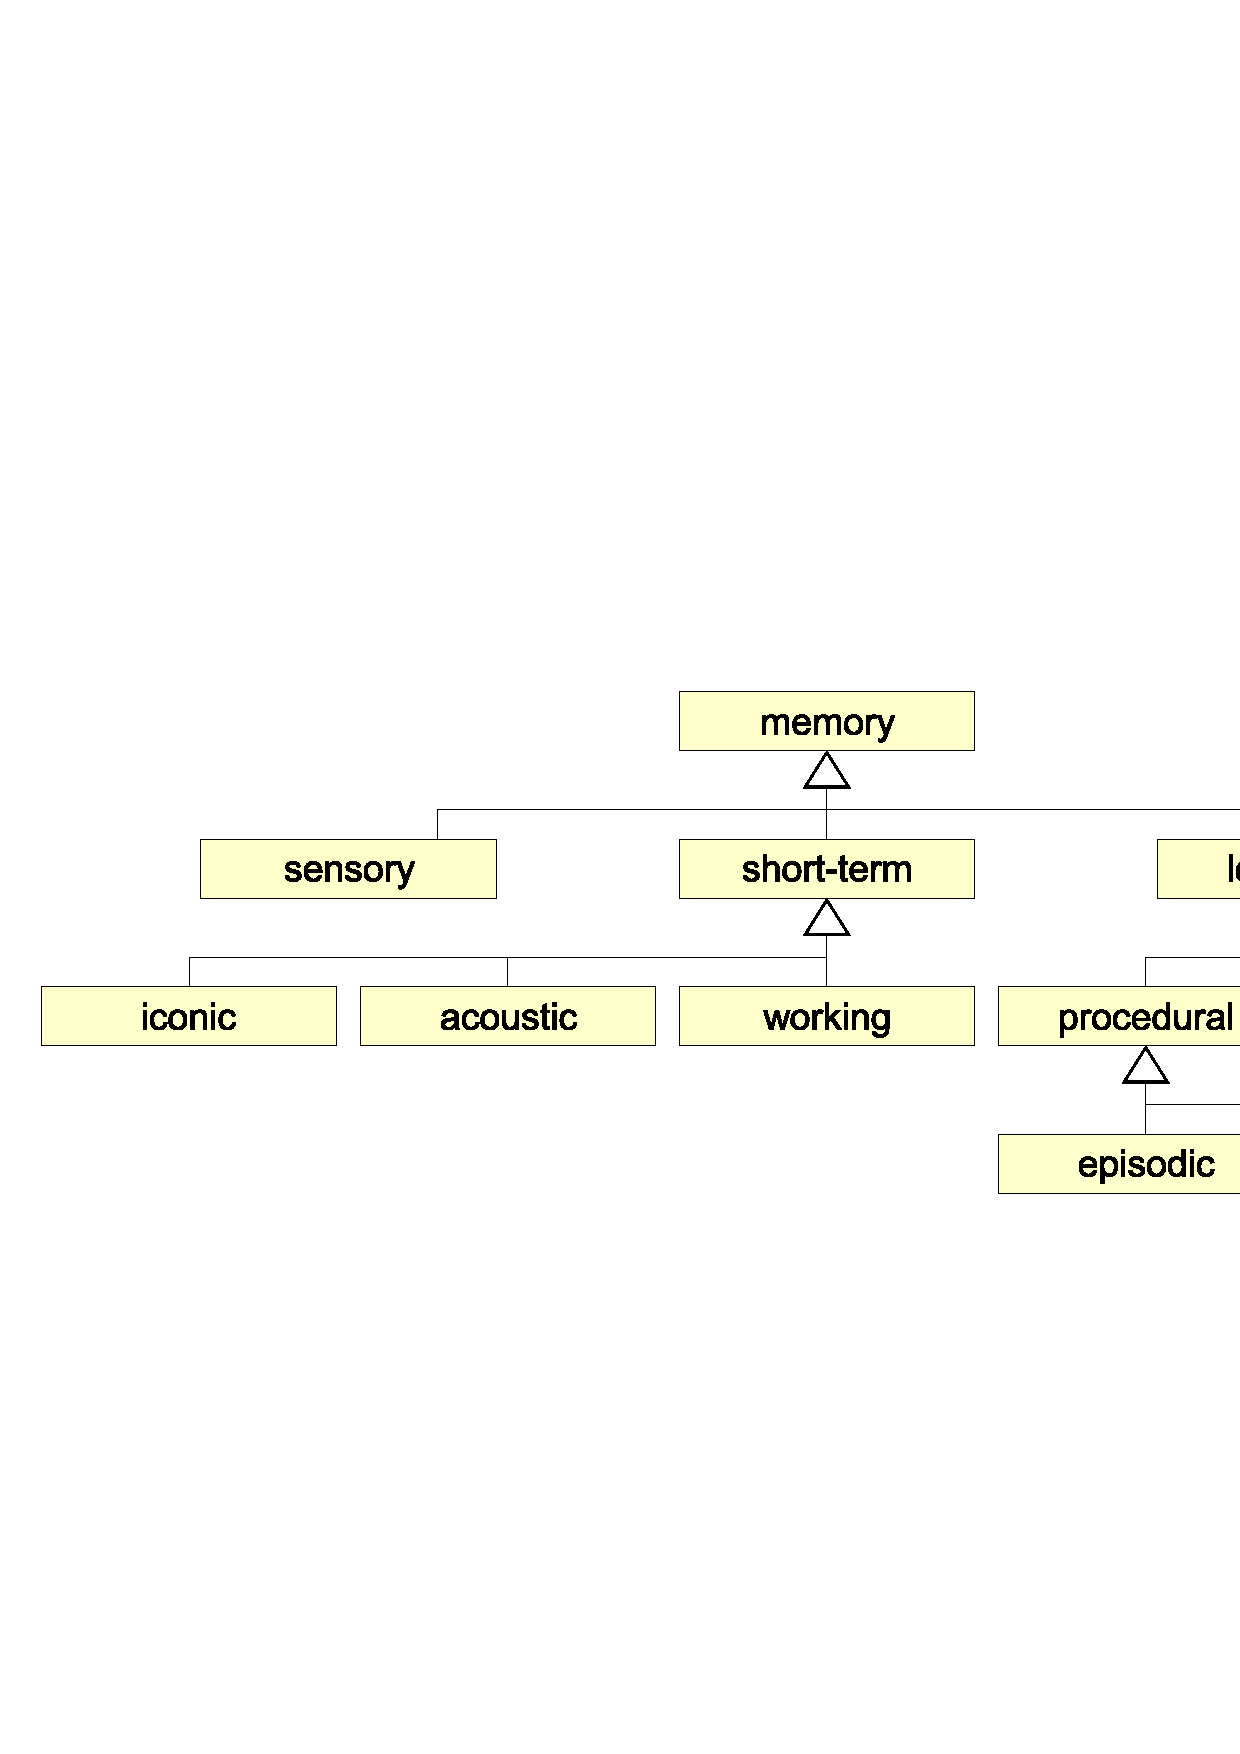
\includegraphics[scale=0.3,angle=-90]{graphic/memory.pdf}
        \caption{Types of Memory \cite{lai, eet}}
        \label{memory_figure}
    \end{center}
\end{figure}

The \emph{Encyclopedia of Educational Technology} (EET) \cite{eet} writes:

\begin{quote}
    The sensory information store has unlimited capacity, and reacts to both
    visual and auditory information. However, the duration of information in
    sensory memory is extremely brief, perhaps only 300 miliseconds, and is
    subject to rapid decay.

    STM, in general, is characterized by a limited capacity of up to seven
    pieces of independent information, and in the brief duration of these items
    in STM, usually anywhere from three to 20 seconds. Additionally, decay
    appears to be the primary mechanism of memory loss in STM.

    LTM efficiently stores our knowledge about the world. It is important to
    contrast LTM with other types of memory and understand how it is
    structured. The knowledge we store in LTM affects our perceptions of the
    world, and influences what information in the environment we attend to. LTM
    provides the framework to which we attach new knowledge, and its properties
    have important implications for instructional design.
\end{quote}

In the words of the Free Wikipedia Encyclopedia \cite{wikipedia}, Information
held in STM may be: \textit{recently processed sensory input; items recently
retrieved from LTM; or the result of recent mental processing.} When doing
mathematical calculations, for example, intermediary results stored in STM are
available for only a short time and forgotten soon after.

The \emph{declarative} LTM is conscious memory, a \emph{film} of past contents
\cite{fernandez}. The \emph{procedural} -- or \emph{non-declarative} -- LTM is
unconscious memory which enables humans to carry out a task (like riding a
bicycle), without having to consciously control it. In other words, procedures
stored in non-declarative LTM are available- and may run as background program.

What effects do these reflections have on the design of software systems? The
storage and dynamic processing of static knowledge may firstly rely on at least
two different kinds of memory, one for \emph{persistent-} and another one for
\emph{transient} storage of knowledge; secondly, they may rely not only on one
main process controlling the system, but (as equivalent to procedural LTM)
employ a number of background processes solving special tasks.

%
% $RCSfile: information_processing_model.tex,v $
%
% Copyright (C) 2002-2008. Christian Heller.
%
% Permission is granted to copy, distribute and/or modify this document
% under the terms of the GNU Free Documentation License, Version 1.1 or
% any later version published by the Free Software Foundation; with no
% Invariant Sections, with no Front-Cover Texts and with no Back-Cover
% Texts. A copy of the license is included in the section entitled
% "GNU Free Documentation License".
%
% http://www.cybop.net
% - Cybernetics Oriented Programming -
%
% http://www.resmedicinae.org
% - Information in Medicine -
%
% Version: $Revision: 1.1 $ $Date: 2008-08-19 20:41:07 $ $Author: christian $
% Authors: Christian Heller <christian.heller@tuxtax.de>
%

\subsection{Information Processing Model}
\label{information_processing_model_heading}
\index{Information Processing Model}
\index{Chunking}

Information processing, from the view of \emph{Cognitive Psychology}, follows
the model shown in figure \ref{processing_figure}. General information has to
pass several stages before it becomes meaningful knowledge. The results of
processing stages are stored in different memories.

\begin{figure}[ht]
    \begin{center}
        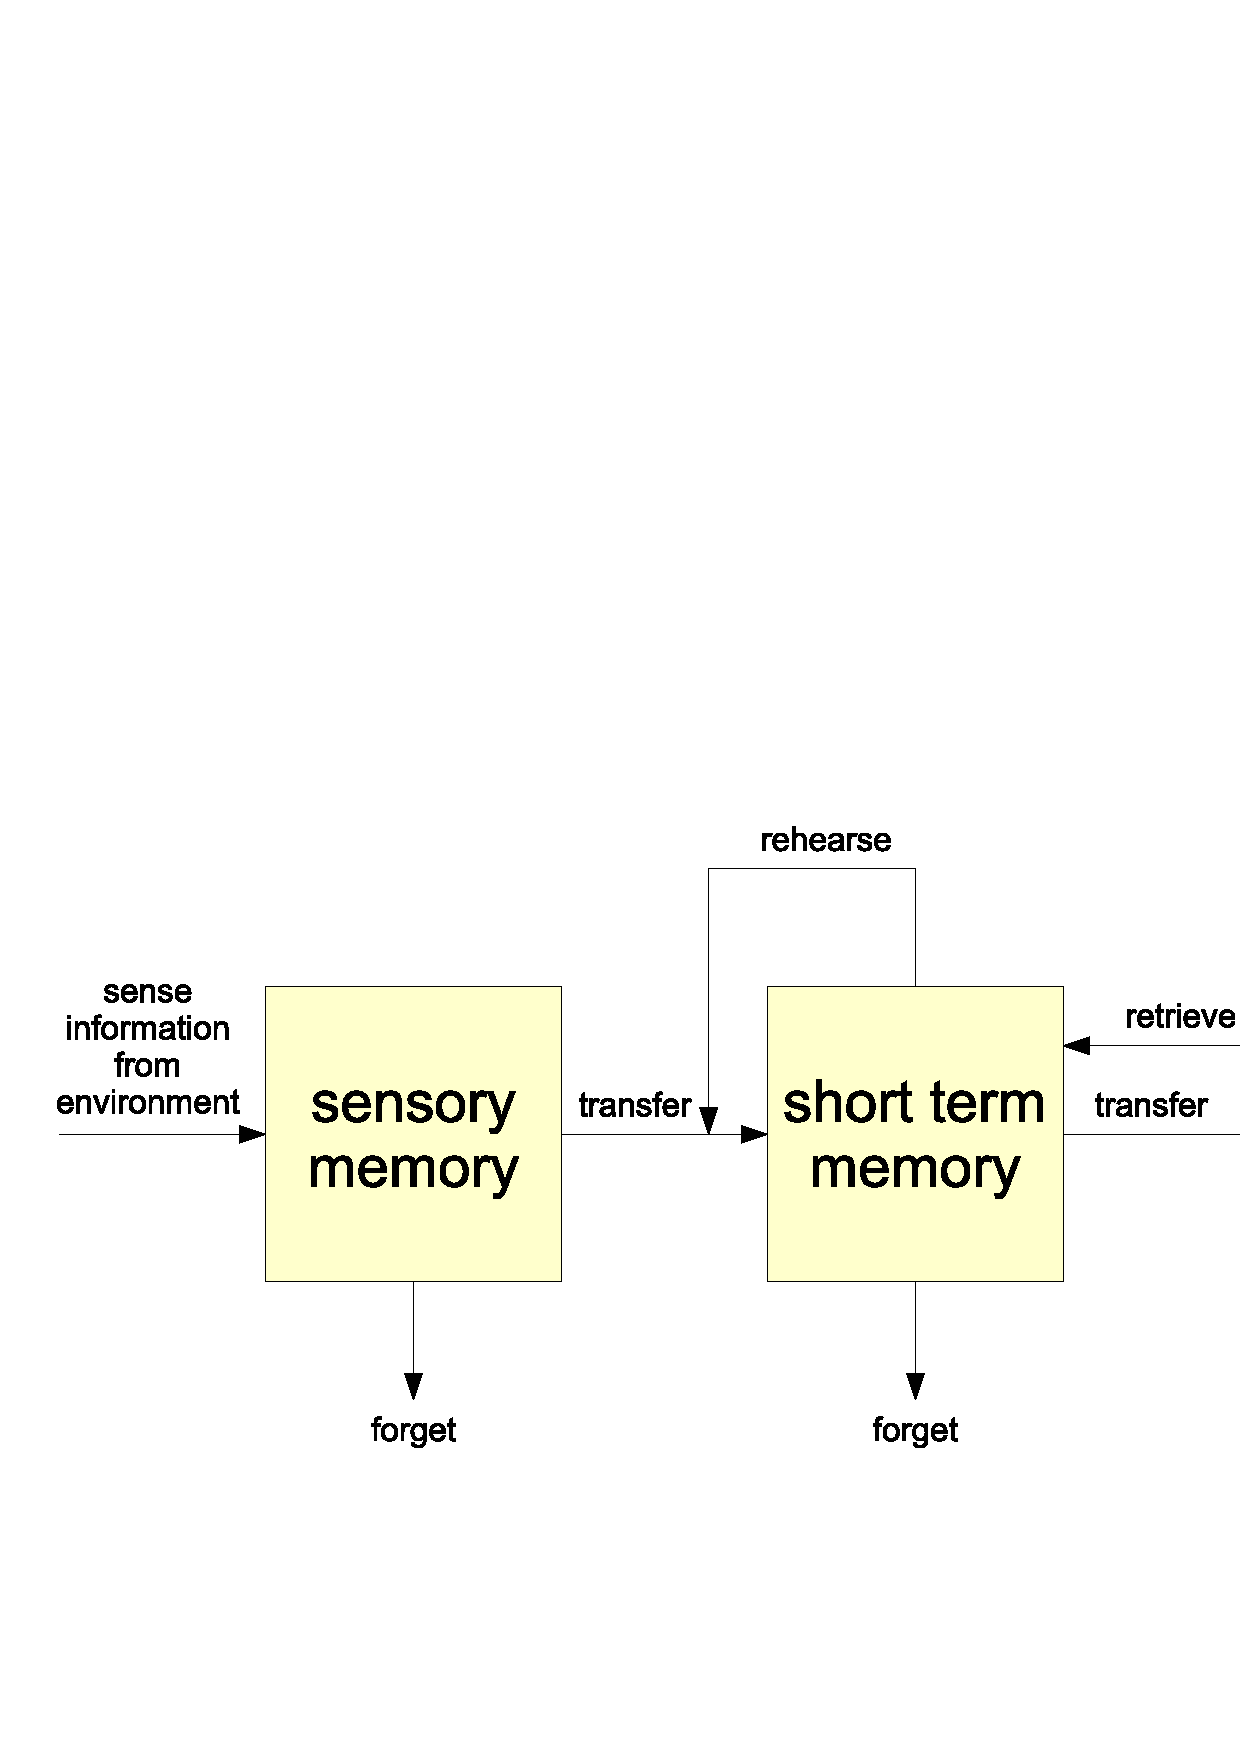
\includegraphics[scale=0.3,angle=-90]{graphic/processing.pdf}
        \caption{Information Processing Model \cite{eet}}
        \label{processing_figure}
    \end{center}
\end{figure}

The \emph{Encyclopedia of Educational Technology} (EET) \cite{eet} writes on
this:

\begin{quote}
    After entering sensory memory, a limited amount of information is
    transferred into short-term memory. \ldots\ The process of transferring
    information from STM into LTM involves the \emph{Encoding} or
    \emph{Consolidation} of information. \ldots\ Recent research (focuses) on
    the necessity of the brain to organise complex information in STM
    \emph{before} it can be encoded into LTM.

    In this process of organization, the \emph{Meaningfulness} or
    \emph{Emotional Content} of an item may play a greater role in its
    retention into LTM. Also, on a more concrete level, the use of
    \emph{Chunking} has been proven to be a significant aid to STM transfer to
    LTM. Because STM's capacity is limited to seven items, regardless of the
    complexity of those items, chunking allows the brain to automatically group
    certain items together.
\end{quote}

Certainly, the emotional content of an item can be neglected for computer
systems as of today. But chunking as a technique to divide information into
discrete items is of great importance in human thinking, which gets
investigated closer in chapter \ref{knowledge_schema_heading}.

%
% $RCSfile: persistent_and_transient.tex,v $
%
% Copyright (C) 2002-2008. Christian Heller.
%
% Permission is granted to copy, distribute and/or modify this document
% under the terms of the GNU Free Documentation License, Version 1.1 or
% any later version published by the Free Software Foundation; with no
% Invariant Sections, with no Front-Cover Texts and with no Back-Cover
% Texts. A copy of the license is included in the section entitled
% "GNU Free Documentation License".
%
% http://www.cybop.net
% - Cybernetics Oriented Programming -
%
% http://www.resmedicinae.org
% - Information in Medicine -
%
% Version: $Revision: 1.1 $ $Date: 2008-08-19 20:41:08 $ $Author: christian $
% Authors: Christian Heller <christian.heller@tuxtax.de>
%

\subsection{Persistent and Transient}
\label{persistent_and_transient_heading}
\index{Integrated Circuit}
\index{IC}
\index{Read Only Memory}
\index{ROM}
\index{Basic Input/ Output System}
\index{BIOS}
\index{Personal Digital Assistant}
\index{PDA}
\index{Electrically Erasable Programmable ROM}
\index{EEPROM}
\index{Flash ROM}
\index{Hard Disk Drive}
\index{HDD}
\index{Random Access Memory}
\index{RAM}
\index{Persistent Data}
\index{Transient Data}
\index{Volatile Data}
\index{Central Processing Unit}
\index{CPU}

In the science of \emph{Informatics}, there are a few \emph{Integrated Circuits}
(IC) -- so-called \emph{Read Only Memories} (ROM) -- containing unchangeable
programs. The \emph{Basic Input/ Output System} (BIOS) of a computer is one
example for such programs, software of \emph{Personal Digital Assistants} (PDA)
or \emph{Mobile Phones} are others. Often, the BIOS is stored in
\emph{Electrically Erasable Programmable ROM} (EEPROM) or its later form called
\emph{Flash ROM}. It thereby gets writable. When writing it, the complete old
BIOS gets overwritten. Most software programs, however, reside on a
\emph{Hard Disk Drive} (HDD) as permanent storage medium.

In order to use them, such \emph{persistent} programs often need to be loaded
into an IC called \emph{Random Access Memory} (RAM) which, other than a ROM,
can be both read from and written to. Most RAMs are \emph{volatile} which means
that the data they store -- to which also belong programs -- are
\emph{transient}, that is get lost in case the computer is powered down. The
ability to manipulate data in memory is a pre-requisite to usefully work with a
computer.

One surely could, with some effort, rearchitect computers so to let the
\emph{Central Processing Unit} (CPU) communicate directly with persistent
memory (like a HDD), instead of RAM. One reason for not doing this is the
\emph{Performance} of computer systems -- RAM can be accessed much faster than a
HDD. Another reason is the independence from differing HDD designs.

What this section by its remarks tries to show is that \emph{static} software
becomes \emph{dynamic}, that is changeable over time, when being loaded into a
RAM whose data (represented by its state) can be processed (manipulated)
through a CPU. Although not being so new, this statement has importance for
some considerations later in this chapter.

While some kinds of software (like standard- or business applications) mainly
\emph{contain} static knowledge of a special domain, other kinds do mainly
\emph{use} that knowledge to dynamically control hardware. The point is that
traditionally, both kinds of software are mixed up. A business application has
to care about memory allocation, graphical input and output (even when using a
framework for that), communication mechanisms and more, although these are not
in its original interest. On the other hand, an operating system often contains
configuration knowledge about its structure or available devices that does not
actually belong into it. In order to achieve a clearer structure with less
dependencies and more flexibility, it is necessary to treat both kinds of
software differently.

